\documentclass[conference]{IEEEtran}
\IEEEoverridecommandlockouts
% The preceding line is only needed to identify funding in the first footnote. If that is unneeded, please comment it out.
\usepackage[portuges,brazil,english]{babel}
\usepackage[utf8]{inputenc}
\usepackage{amsmath,amssymb,amsfonts}
\usepackage{algorithmic}
\usepackage{graphicx}
\usepackage{textcomp}
\usepackage{float}
\def\BibTeX{{\rm B\kern-.05em{\sc i\kern-.025em b}\kern-.08em
    T\kern-.1667em\lower.7ex\hbox{E}\kern-.125emX}}

\usepackage{subcaption}
\usepackage[style=mla,guessmedium=false,backend=bibtex]{biblatex}
\addbibresource{report.bib}

\begin{document}

\renewcommand{\figurename}{Fig.}
\renewcommand{\refname}{Referências}

\title{Regressão Logística e Redes Neurais para Classificação de Vestuário (Fashion MNIST)}

\author{\IEEEauthorblockN{Carolina F. Cuba}
\IEEEauthorblockA{
226004 \\
carolinacuba23@gmail.com}
\and
\IEEEauthorblockN{Leonardo de Melo Joao}
\IEEEauthorblockA{
228118 \\
l228118@g.unicamp.br}}

\maketitle

\section{Introdução}	
	Detecção de doenças em imagens médicas, análise de genômas e análise sentimento em redes sociais são exemplos de problemas atuais que possuem dados tão volumósos e complexos que só podem ser solucionados com o auxílio de ferramentas capazes de extrair padrões significativos desses dados. Atualmente, os algorítmos mais bem sucedidos para essa tarefa são as Redes Neurais Artificiais (ANN, do inglês Artificial Neural Networks).
	
	Embora na maioria dos casos são necessárias Redes Neurais extremamente complexas e que demandam grande poder computacional (Redes Neurais Profundas), o funcionamento dessas redes complexas se assemelha muito ao de suas versões mais simples. Sabendo disso, o intuito desse projeto é estudar de maneira didática o funcionamento de versões mais simples desse algorítmo.
	
	Para tanto, apresentaremos duas versões simples de Redes Neurais e duas versões de Regressões Logísticas, que é o algoritmo que originou a base do funcionamento dos neurônios.
	
	Ambas versões de ambos algorítmos serão testados na base de dados Fashion MNIST. O objetivo é, dada uma imagem de vestuário, classificá-la em 1 dentre 10 possíveis classes. As métricas utilizadas para verificação de performance dos modelos foram: precision, recall e f1-score.
	
\section{Conjunto de Dados: Fashion MNIST}

	A Fashion MNIST, proposta por \citeauthor{xiao2017/online} (\citeyear{xiao2017/online}), é uma base criada especialmente para benchmarking de algorítmos de machine learning, como informado pelo próprio autor.
	
	O desafio é classificar as imagens que a compõe entre 10 posśiveis classes de vestuário, sendo elas: [0] Camiseta ("T-shirt/top"); [1] Calça ("Trouser"); [2] Pullover; [3] Vestido ("Dress"); [4] Casaco ("Coat"); [5] Sandália ("Sandal"); [6] Camisa ("Shirt"); [7] Tênis ("Sneaker"); [8] Bolsa ("Bag"); [10] Bota ("Ankle boot").
	
	Cada imagem possui 28x28 pixels e são em tons de cinza, ou seja, cada imagem possui um vetor inicial de características de tamanho $28*28*1 = 784$, onde 1 é o número de bandas de uma imagem em escala de cinza.
	
	A base é composta por 60.000 imagens para treinamento e 10.000 para teste. As imagens de teste só foram utilizadas depois de apenas um modelo ser escolhido. Para escolher esse modelo, testes de validação foram realizados no conjunto de trainamento que, por sua vez, foi dividido com 70\% para treino e 30\% para validação.
	
\section{Regressão Logística}

\subsection{One versus All}

\subsection{Softmax}

\section{Redes Neurais Artificiais}

	Como um exemplo de computação bio inspirada, as Redes Neurais Artificiais são uma abstração computacional para representação de um modelo cerebral. Para tanto, neurônios foram modelados por	\citeauthor{rosenblatt1957perceptron} (\citeyear{rosenblatt1957perceptron}) como perceptrons. Apesar desse modelo ser mais facilmente relacionado a um neurônio, seu funcionamento é igual de uma regressão logística: um conjunto de dados ponderados por um vetor de pesos entram em um perceptron, são combinados e submetidos à uma função de ativação. Quando o valor de saída da função de ativação é maior que zero é dito que o perceptron ativou. Essa representação do perceptron pode ser vista na Figura 1.
	
  \begin{figure}[!h]
      \centering
      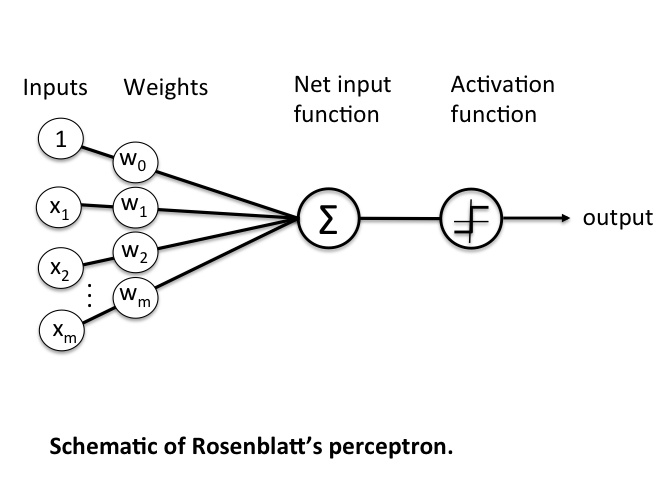
\includegraphics[width=0.6\columnwidth]{images/perceptron.png}
      \caption{Perceptron de Rosenblatt}
      \label{fig1}
  \end{figure}
  
  Em linhas gerais, uma Rede Neural é um conjunto de perceptrons interconectados onde a saída de um conjunto de perceptrons é ponderada por um vetor de pesos e dada como entrada de outro conjunto de perceptrons. Essa estrutura é chamada de MLP (Perceptron multicamadas, do inglês Multi Layer Perceptron), onde cada conjunto de perceptrons é uma camada da rede.
  
  A camada de entrada (Input Layer) envia os dados de entrada ponderados pelos seus respectivos pesos para a camada escondida (Hidden Layer). Em sequência, cada neurônio da camada escondida combina seus valores de entrada e os submete a uma função de ativação. O resultado das ativações é enviado ou a uma camada de saída (Output Layer) ou a outra camada escondida que repete o mesmo processo da camada anterior. A ativação da camada de saída é o que define a classe na qual o objeto de entrada pertence. Uma rede com muitas camadas escondidas é chamada de DNN (Rede Neural Profunda, do inglês Deep Neural Network).
  
  A quantidade de camadas escondidas e de neurônios em cada camada pode variar dependendo da complexidade do problema. Nesse trabalho, esses parâmetros foram definidos de maneira empírica, bem como o valor da constante de aprendizagem \textit{learning rate}).
  
  Originalmente, a classificação nas redes neurais é binária. Isso quer dizer que a rede só é capaz de classificar se a entrada é de uma classe ou não. Assim como na regressão logística, para resolver problemas multiclasse, utiliza-se a função softmax como função de ativação da camada de saída.
  
  Contudo, as MLPs só puderam ser utilizadas devido a uma técnica de aprendizagem baseado no erro retropropagado pelas camadas, proposta por \citeauthor{rumelhart1986learning} (\citeyear{rumelhart1986learning}). O problema resolvido foi o de como se atualizar os pesos das camadas mais distântes à camada de saída. O algorítmo de retropropagação baseia-se em derivadas subsequentes pela regra da cadeia, propagando o erro para as camadas mais distantes, identificando a relevância de cada peso no erro final. Isso permite os valores dos pesos serem alterados baseados na sua influência no erro final e em quão grande foi o erro. Em linha gerais, o valor de um peso seria alterado significantemente se o erro for alto e se esse peso foi importante no calculo da classificação que causou o erro. Essa técnica é conhecida como Backpropagation (retropropagação) e uma boa explicação do seu passo a passo pode ser vista em: https://theclevermachine.wordpress.com/2014/09/06/derivation-error-backpropagation-gradient-descent-for-neural-networks/.
  
  Apesar da explicação ter sido breve, o restante desse trabalho será utilizado para descrever alguns detalhes e escolhas de implementação, demonstrando os efeitos dessas escolhas nos testes realizados para escolher um modelo.
  
\section{Funções de ativação}
	Antes dos testes serem apresentados, faz-se necessário uma breve descrição das 3 funções de ativação implementadas: [1] sigmoid; [2] tangente hiperbólica; [3] rectified linear unit (ReLU).
	
\subsection{Sigmoid}

	A sigmoid é primeira função a ser implementada em um perceptron, vindo de herânça da regressão logística. Ela é uma função descrita pela equação: 

\begin{equation}
sigmoid(x) = \dfrac{1}{1 + e^{-x}}
\end{equation}	

	O problema dessa função é que os valores de saída estão entre 0 e 1. Isso causa problemas no calculo da descida de gradiente uma vez que devido aos valores de saída serem sempre baixos, os valores dos pesos variam muito pouco nas suas atualizações. Esse problema é chamado de \textit{vanishing gradient}
	
	Para a atualização de parâmetros, a derivada dessa função deve ser utilizada durante o backpropagation. A derivada da sigmoid é descrita pela equação:
	

\begin{equation}
\dfrac{d}{dx}sigmoid(x) = \dfrac{1}{1 + e^{-z}} * (1 - \dfrac{1}{1 + e^{-z}})
\end{equation}	

\subsection{Tangente Hiperbólica}
  
	A tangente hiperbólica (representada geralmente como tanh), é similar à sigmoid, mas seus valores variam entre -1 e 1. Entretanto, ela ainda apresenta o problema do \textit{vanishing gradient}. A tanh é definida pela equação:
  
\begin{equation}
tanh(x) = \dfrac{2}{1+e^{-2x}} - 1
\end{equation}

	Sua derivada, utilizada no backpropagation, é definida por:
\begin{equation}
\dfrac{d}{dx}tanh(x) =  1 - (\dfrac{2}{1+e^{-2x}} - 1)^2
\end{equation}	

\subsection{Rectified Linear Unit (ReLU)}

	Para resolver o problema do vanishing gradient, \citeauthor{nair2010rectified} (\citeyear{nair2010rectified}) propôs a ReLU. Essa função é definida como 0 quando $x	\leq 0$ e $x$ quando $x>0$. Isso faz com que os valores tenham um peso maior no algoritmo do gradiente descendente. Sua representação matemática é:
	
\begin{equation}
ReLU(x) =  max(0,x)
\end{equation}

	Sua derivada, utilizada na backpropagation, é 1 quando $x>0$ e 0 quando $x \leq 0$.
	
\section{Criando e escolhendo os modelos}

\subsection{Regressão Logística}

\subsubsection{One versus All}

\subsubsection{Softmax}

\subsection{Rede Neural}

	Começamos implementando uma Rede Neural com apenas 1 camada escondida. Todos os testes foram feitos com 3000 épocas, valor utilizado para manter um tempo de execução aceitável. Os valores da constante de aprendizagem, do número de neurônios e a função de ativação utilizada foram atribuídos empiricamente e seus respectivos testes estão descritos nas subções seguintes.
	
	Como a linguagem de programação escolhida foi Python, as operações de Feedforward e Backpropagation foram implementadas de maneira vetorizada uma vez que a linguagem não lida bem com estruturas de repetições explicitas. Com isso, o tempo de execução foi razoavelmente rápido.
	
	As métricas de comparação dos modelos foram: precision, que mede quantas das amostras preditas como da classe $x$ realmente eram daquela classe; recall, que mede quantas das amostras da classe $x$ foram corretamente preditas como $x$; e o f1-score é uma combinação das outras duas métricas.
	
	Os primeiros testes executados com todas as funções de ativação foram nessa versão da rede. As funções sigmoid e tanh estavam funcionando corretamente e convergindo para um erro mínimo. Entretanto quando a relu era aplicada os valores dos pesos começavam a tender para infinito positivo e negativo.
	
	Após alguns testes e pesquisas, descobrimos que quando utiliza-se relu o valor inicial dos pesos não podem ser muito elevados, uma vez que esse valor não é normalizado entre $(0,1)$ ou entre $(-1,1)$ como é o caso na sigmoid e na tanh.
	
	Nesse cenário, os valores dos pesos foram inicializados com valores menores que $1*10^{-2}$. Com essa alteração, todas funções de ativação começaram a convergir para o mínimo e os testes puderam ser feitos.

\subsubsection{Uma camada escondida}
	
	A Tabela 1 mostra alguns dos testes executados. Antes desses testes o learning rate já tinha sido testados com valores menores e mostrava necessitar muitas iterações para convergir para valores próximos. Note que NHL na tabela é o número de neurônios na camada escondida.
	
\begin{table}[h!]
 \begin{center}
  \caption{Testes de Performance para NN com 1 Camada Oculta}
  \label{table:table1}
  \begin{tabular}{ |c|c|c|c|c|c|c| }
   \hline
   Ativação & LR & NHL & Precision & Recall & F1-Score & Tempo(s)\\
   \hline
   ReLU & 0.3 & 16 & 0.86 & 0.87 & 0.86 & 142.2 \\ 
                   & 0.1 & 16 & 0.85 & 0.86 & 0.85 & 166.1 \\
                   & 0.4 & 16 & 0.86 & 0.86 & 0.86 & 170.4 \\
                   & 0.3 & 32 & 0.87 & 0.88 & 0.87 & 233.4 \\
                   & 0.4 & 32 & 0.87 & 0.88 & 0.87 & 234.5 \\
   \hline
   Sigmoid & 0.3 & 16 & 0.85 & 0.85 & 0.85 & 165.6 \\ 
                     & 0.1 & 16 & 0.82 & 0.82 & 0.82 & 200.5 \\
                     & 0.4 & 16 & 0.86 & 0.86 & 0.86 & 196.1 \\
                     & 0.3 & 32 & 0.86 & 0.86 & 0.86 & 294.0 \\
                     & 0.4 & 32 & 0.86 & 0.87 & 0.86 & 293.9 \\	
   \hline
   Tanh & 0.3 & 16 & 0.86 & 0.87 & 0.86 & 159.9 \\ 
                     & 0.1 & 16 & 0.86 & 0.86 & 0.86 & 192.0 \\
                     & 0.4 & 16 & 0.86 & 0.86 & 0.86 & 194.3 \\
                     & 0.3 & 32 & 0.88 & 0.87 & 0.87 & 270.1 \\
                     & 0.4 & 32 & 0.87 & 0.87 & 0.87 & 284.2 \\

 \hline
 \end{tabular}
 \end{center}
\end{table}

	Nos testes feitos, o modelo que obteve os melhores resultados foi o que utilizava Relu, learning rate de 0.3 e 32 neurônios na camada escondida. Além disso, a ReLU obteve os melhores resultados em tempo, com a sigmoid sendo a mais lenta e com piores resultados.
	
	A tanh teve resultados bem próximos aos da ReLU mas levou mais tempo para executar.

\subsubsection{Duas camadas ocultas}

	Na rede com duas camadas ocultas com 16 neurônios em cada camada e learning rate 0.3, o valor dos custos a cada época não convergia sempre para o mínimo, saltando entre erros mais altos e mais baixos. Por conta disso, resolvemos experimentar com learning rates mais baixos.
	
	Com os learning rates menores, o valor dos custos desceu continuamente. Porém, 3000 iterações não pareceu ser o suficiente para que a rede convergisse o necessário. Dito isso, o melhor modelo provavelmente seria outro caso o tempo de execução não tivesse sido pré-determinado. Infelizmente devido à data de submissão não pudemos realizar todos testes necessários.
	
	O problema descrito acima só ocorreu nas redes com 16 neurônios em ambas camadas. Por conta disso, nos demais casos o learning rate foi mantido mais alto.

\begin{table}[h!]
 \begin{center}
  \caption{Testes de Performance para NN com 1 Camada Oculta}
  \label{table:table1}
  \begin{tabular}{ |c|c|c|c|c|c|c| }
   \hline
   Ativação & LR & NHL1 & NHL2 & Precision & Recall & F1-Score & Tempo(s)\\
   \hline
   ReLU & 0.3 & 16 & 16 & 0.84 & 0.85 & 0.84 & 199.1 \\
        & 0.2 & 16 & 16 & 0.84 & 0.85 & 0.84 & 194.75 \\
        & 0.1 & 16 & 16 & 0.84 & 0.84 & 0.84 & 194.1 \\
        & 0.1 & 32 & 16 & 0.85 & 0.85 & 0.84 & 256.0 \\
        & 0.3 & 32 & 16 & 0.86 & 0.87 & 0.86 & 274.5 \\
        & 0.3 & 16 & 32 & 0.85 & 0.85 & 0.84 & 256.0 \\
        & 0.1 & 32 & 32 & 0.87 & 0.87 & 0.86 & 287.2 \\
        & 0.3 & 32 & 32 & 0.86 & 0.86 & 0.86 & 319.5 \\
                   & 0.4 & 16 & 0.86 & 0.86 & 0.86 & 170.4 \\
                   & 0.3 & 32 & 0.87 & 0.88 & 0.87 & 233.4 \\
                   & 0.4 & 32 & 0.87 & 0.88 & 0.87 & 234.5 \\
   \hline
   Sigmoid & 0.3 & 16 & 0.85 & 0.85 & 0.85 & 165.6 \\ 
                     & 0.1 & 16 & 0.82 & 0.82 & 0.82 & 200.5 \\
                     & 0.4 & 16 & 0.86 & 0.86 & 0.86 & 196.1 \\
                     & 0.3 & 32 & 0.86 & 0.86 & 0.86 & 294.0 \\
                     & 0.4 & 32 & 0.86 & 0.87 & 0.86 & 293.9 \\	
   \hline
   Tanh & 0.3 & 16 & 0.86 & 0.87 & 0.86 & 159.9 \\ 
                     & 0.1 & 16 & 0.86 & 0.86 & 0.86 & 192.0 \\
                     & 0.4 & 16 & 0.86 & 0.86 & 0.86 & 194.3 \\
                     & 0.3 & 32 & 0.88 & 0.87 & 0.87 & 270.1 \\
                     & 0.4 & 32 & 0.87 & 0.87 & 0.87 & 284.2 \\

 \hline
 \end{tabular}
 \end{center}
\end{table}
	
\section{Testando o modelo final no Fashion MNIST}

\printbibliography

\end{document}